Ở mức thiết kế logic (\textit{Logical Design Level}), mục tiêu cốt lõi là chuyển hóa mô hình dữ liệu quan niệm trừu tượng (ERD/UML) thành lược đồ quan hệ lô-gíc (\textit{Logical Relational Schema}) cụ thể, xác định rõ cấu trúc các bảng, cột, khóa chính (PK), khóa ngoại (FK) và các ràng buộc toàn vẹn [1, 2]. Đồ án áp dụng \textbf{Thuật toán 2.2} (\textit{Algorithm 2.2: Ánh xạ ERD sang Lược đồ Quan hệ}) để đảm bảo tính toàn vẹn tham chiếu, loại bỏ các dị thường dữ liệu và đưa toàn bộ lược đồ đạt tiêu chuẩn chuẩn hóa 3NF cho hệ thống \textbf{LivingDocs — Design and Implementation of an AI-Assisted Self-Updating Document System for Engineering Teams} [3-5].

Quá trình này tiếp nhận đầu vào (\textit{Input}) là Sơ đồ Quan niệm (\textit{Conceptual ERD/UML}) đã qua kiểm chứng ở Stage 1, và kết xuất đầu ra (\textit{Output}) là Lược đồ Quan hệ Lô-gíc (\textit{Logical Schema}) hoàn chỉnh, hồ sơ Ràng buộc Khóa ngoại/Giá trị miền (\textit{FK \& CHECK Rules}) và Báo cáo chứng minh Chuẩn hóa 3NF [3, 5-12].

\textbf{Quy trình Thuật toán 2.2 (\textit{Relational Mapping Algorithm}):}
\begin{itemize}
    \item \textbf{Đầu vào (\textit{Input}):} Sơ đồ Quan niệm ERD/UML và từ điển dữ liệu hoàn chỉnh từ Stage 1.
    \item \textbf{Bước 1 (Thực thể mạnh):} Ánh xạ các thực thể mạnh thành các bảng chính, chuyển thuộc tính đơn thành cột và thiết lập Khóa chính (PK).
    \item \textbf{Bước 2 (Thực thể yếu):} Ánh xạ các thực thể yếu thành các bảng phụ thuộc, gán Surrogate PK kiểu UUID và cài đặt FK trỏ về thực thể chủ.
    \item \textbf{Bước 3 \& 4 (Mối kết hợp $1:1$ và $1:N$):} Chèn Khóa ngoại (FK) từ bảng phía 1 sang bảng phía $N$ (hoặc phía tham gia bắt buộc) kèm các ràng buộc NOT NULL/UNIQUE phù hợp.
    \item \textbf{Bước 5 (Mối kết hợp $M:N$):} Khởi tạo các bảng trung gian (\textit{Junction Tables}) chứa cặp Khóa ngoại (FK) trỏ về hai bảng gốc và các thuộc tính riêng của mối kết hợp.
    \item \textbf{Bước 6 (Thuộc tính đặc biệt):} Phẳng hóa các thuộc tính phức hợp thành các cột đơn độc lập và tách các thuộc tính đa trị thành các bảng phụ riêng.
    \item \textbf{Bước 7 (Ràng buộc \& Chuẩn hóa):} Khai báo tập Phụ thuộc hàm (FDs), chứng minh lược đồ đạt chuẩn 3NF và thiết lập các ràng buộc toàn vẹn (\textit{FK Constraints}).
    \item \textbf{Đầu ra (\textit{Output}):} Lược đồ Quan hệ Lô-gíc (\textit{Logical Schema}) hoàn chỉnh đạt chuẩn 3NF và hồ sơ ràng buộc toàn vẹn.
\end{itemize}

\section{ Ánh xạ Thực thể, Mối kết hợp \& Phẳng hóa Thuộc tính (Thuật toán 2.2) }



\subsubsection*{Bước 1: Thực thể mạnh $\rightarrow$ Bảng chính}
Chuyển 7 thực thể mạnh thành 7 bảng chính, đặt tên theo chuẩn \texttt{snake\_case} số nhiều:
\begin{itemize}
    \item \texttt{users}, \texttt{workspaces}, \texttt{roles}, \texttt{permissions}, \texttt{repositories}, \texttt{templates}, \texttt{documents}.
\end{itemize}

\subsubsection*{Bước 2: Thực thể yếu $\rightarrow$ Bảng phụ \& Mối kết hợp $M:N \rightarrow$ Bảng trung gian (Surrogate PK UUID)}
Chuyển 16 thực thể yếu thành 16 bảng phụ, mỗi bảng được gán khóa chính nhân tạo (Surrogate PK) kiểu \texttt{UUID} độc lập với bảng cha, mang FK định danh (identifying FK) trỏ về đúng 1 bảng cha:
\begin{itemize}
    \item \texttt{github\_connections} (phụ thuộc \texttt{users})
    \item \texttt{branches} (phụ thuộc \texttt{repositories})
    \item \texttt{commits} (phụ thuộc \texttt{branches}; FK phụ \texttt{author\_user\_id} $\rightarrow$ \texttt{users}, \texttt{pr\_id} $\rightarrow$ \texttt{pull\_requests})
    \item \texttt{pull\_requests} (phụ thuộc \texttt{repositories})
    \item \texttt{code\_diffs} (phụ thuộc \texttt{commits})
    \item \texttt{files} (phụ thuộc \texttt{repositories})
    \item \texttt{code\_entities} (phụ thuộc \texttt{files})
    \item \texttt{template\_sections} (phụ thuộc \texttt{templates})
    \item \texttt{placeholders} (phụ thuộc \texttt{template\_sections})
    \item \texttt{document\_versions} (phụ thuộc \texttt{documents})
    \item \texttt{change\_logs} (phụ thuộc \texttt{document\_versions})
    \item \texttt{reviews} (phụ thuộc \texttt{document\_versions}; FK phụ \texttt{reviewer\_user\_id} $\rightarrow$ \texttt{users})
    \item \texttt{review\_comments} (phụ thuộc \texttt{reviews})
    \item \texttt{approvals} (phụ thuộc \texttt{document\_versions}; FK phụ \texttt{approver\_user\_id} $\rightarrow$ \texttt{users})
    \item \texttt{grounding\_evidences} (phụ thuộc \texttt{document\_versions})
    \item \texttt{drift\_alerts} (phụ thuộc \texttt{grounding\_evidences})
\end{itemize}

Song song đó, chuyển các mối kết hợp $M:N$ (bao gồm 1 mối kết hợp 3 ngôi và 1 mối kết hợp đệ quy) thành 6 bảng trung gian, mỗi bảng được gán Surrogate PK riêng kiểu \texttt{UUID}, chứa tối thiểu 2 FK cùng vai trò định danh trỏ về các bảng gốc:
\begin{itemize}
    \item \texttt{workspace\_members} (mối kết hợp 3 ngôi \textit{participates}: \texttt{user\_id}, \texttt{workspace\_id}, \texttt{role\_id})
    \item \texttt{role\_permissions} (mối kết hợp \textit{contains}: \texttt{role\_id}, \texttt{permission\_id})
    \item \texttt{commit\_file} (mối kết hợp \textit{modifies}: \texttt{commit\_id}, \texttt{file\_id})
    \item \texttt{dependencies} (mối kết hợp đệ quy \textit{depends\_on}: \texttt{dependent\_entity\_id}, \texttt{target\_entity\_id} --- cả hai cùng trỏ về \texttt{code\_entities})
    \item \texttt{template\_mappings} (mối kết hợp \textit{maps\_to}: \texttt{placeholder\_id}, \texttt{code\_entity\_id})
    \item \texttt{grounding\_evidence\_code\_entities} (mối kết hợp \textit{references\_code}: \texttt{evidence\_id}, \texttt{code\_entity\_id})
\end{itemize}

\subsubsection*{Bước 3 \& 4: Quan hệ 1:1, 1:N $\rightarrow$ Chèn FK}
\textbf{Nguyên tắc:} Chuyển khóa chính (PK) của bảng phía 1 sang làm khóa ngoại (FK) ở bảng phía N. Với quan hệ 1:1, đặt khóa ngoại ở phía tham gia tùy chọn và gán ràng buộc \texttt{UNIQUE} để đảm bảo tính một-một.
\begin{itemize}
    \item \texttt{users.user\_id} (PK) $\rightarrow$ \texttt{github\_connections.user\_id} (FK) (1:1 nghiệp vụ, ràng buộc \texttt{UNIQUE})
    \item \texttt{workspaces.workspace\_id} (PK) $\rightarrow$ \texttt{repositories.workspace\_id} (FK) (1:N)
    \item \texttt{repositories.repository\_id} (PK) $\rightarrow$ \texttt{branches.repository\_id} (FK) (1:N)
    \item \texttt{branches.branch\_id} (PK) $\rightarrow$ \texttt{commits.branch\_id} (FK) (1:N)
    \item \texttt{commits.author\_user\_id} (FK) $\rightarrow$ \texttt{users.user\_id} (PK) (1:N)
    \item \texttt{commits.pr\_id} (FK) $\rightarrow$ \texttt{pull\_requests.pr\_id} (PK) (1:N, cho phép NULL)
    \item \texttt{pull\_requests.repository\_id} (FK) $\rightarrow$ \texttt{repositories.repository\_id} (PK) (1:N)
    \item \texttt{code\_diffs.commit\_id} (FK) $\rightarrow$ \texttt{commits.commit\_id} (PK) (1:N)
    \item \texttt{files.repository\_id} (FK) $\rightarrow$ \texttt{repositories.repository\_id} (PK) (1:N)
    \item \texttt{code\_entities.file\_id} (FK) $\rightarrow$ \texttt{files.file\_id} (PK) (1:N)
    \item \texttt{templates.workspace\_id} (FK) $\rightarrow$ \texttt{workspaces.workspace\_id} (PK) (1:N)
    \item \texttt{template\_sections.template\_id} (FK) $\rightarrow$ \texttt{templates.template\_id} (PK) (1:N)
    \item \texttt{placeholders.section\_id} (FK) $\rightarrow$ \texttt{template\_sections.section\_id} (PK) (1:N)
    \item \texttt{documents.workspace\_id} (FK) $\rightarrow$ \texttt{workspaces.workspace\_id} (PK) (1:N)
    \item \texttt{documents.author\_user\_id} (FK) $\rightarrow$ \texttt{users.user\_id} (PK) (1:N)
    \item \texttt{document\_versions.document\_id} (FK) $\rightarrow$ \texttt{documents.document\_id} (PK) (1:N)
    \item \texttt{change\_logs.version\_id} (FK) $\rightarrow$ \texttt{document\_versions.version\_id} (PK) (1:N)
    \item \texttt{reviews.version\_id} (FK) $\rightarrow$ \texttt{document\_versions.version\_id} (PK) (1:N)
    \item \texttt{reviews.reviewer\_user\_id} (FK) $\rightarrow$ \texttt{users.user\_id} (PK) (1:N)
    \item \texttt{review\_comments.review\_id} (FK) $\rightarrow$ \texttt{reviews.review\_id} (PK) (1:N)
    \item \texttt{approvals.version\_id} (FK) $\rightarrow$ \texttt{document\_versions.version\_id} (PK) (1:N)
    \item \texttt{approvals.approver\_user\_id} (FK) $\rightarrow$ \texttt{users.user\_id} (PK) (1:N)
    \item \texttt{grounding\_evidences.version\_id} (FK) $\rightarrow$ \texttt{document\_versions.version\_id} (PK) (1:N)
    \item \texttt{drift\_alerts.evidence\_id} (FK) $\rightarrow$ \texttt{grounding\_evidences.evidence\_id} (PK) (1:N)
\end{itemize}

\subsubsection*{Bước 5: Quan hệ M:N $\rightarrow$ Bảng trung gian}
Tạo 6 bảng trung gian, mỗi bảng có Surrogate PK riêng kiểu \texttt{UUID} và tối thiểu 2 FK trỏ về các bảng gốc:
\begin{itemize}
    \item \texttt{workspace\_members}: chứa FK \texttt{user\_id}, \texttt{workspace\_id}, \texttt{role\_id} (mối kết hợp 3 ngôi \textit{participates}, tỷ lệ M:N:1)
    \item \texttt{role\_permissions}: chứa FK \texttt{role\_id}, \texttt{permission\_id} (mối kết hợp \textit{contains}, M:N)
    \item \texttt{commit\_file}: chứa FK \texttt{commit\_id}, \texttt{file\_id} (mối kết hợp \textit{modifies}, M:N)
    \item \texttt{dependencies}: chứa FK \texttt{dependent\_entity\_id}, \texttt{target\_entity\_id} (mối kết hợp đệ quy \textit{depends\_on}, M:N)
    \item \texttt{template\_mappings}: chứa FK \texttt{placeholder\_id}, \texttt{code\_entity\_id} (mối kết hợp \textit{maps\_to}, M:N)
    \item \texttt{grounding\_evidence\_code\_entities}: chứa FK \texttt{evidence\_id}, \texttt{code\_entity\_id} (mối kết hợp \textit{references\_code}, M:N)
\end{itemize}

\subsubsection*{Bước 6: Thuộc tính đặc biệt}
\begin{itemize}
    \item \textbf{Phẳng hóa thuộc tính phức hợp:}
    \begin{itemize}
        \item \texttt{User.FullName} $\rightarrow$ \texttt{users.first\_name}, \texttt{users.last\_name}
        \item \texttt{Commit.AuthorInfo} $\rightarrow$ \texttt{commits.author\_name}, \texttt{commits.author\_email}
        \item \texttt{CodeEntity.position} $\rightarrow$ \texttt{code\_entities.start\_line}, \texttt{code\_entities.end\_line}
    \end{itemize}
    \item \textbf{Tách thuộc tính đa trị thành bảng phụ chứa FK trỏ về bảng chính:}
    \begin{itemize}
        \item \texttt{User.NotificationPreferences} $\rightarrow$ \texttt{user\_notification\_preferences}
        \item \texttt{GitHubConnection.scopes} $\rightarrow$ \texttt{github\_connection\_scopes}
        \item \texttt{PullRequest.labels} $\rightarrow$ \texttt{pull\_request\_labels}
    \end{itemize}
\end{itemize};

% ==========================================
\section{ Lược đồ Quan hệ Lô-gíc (Logical Schema) \& 3NF-Phân hệ Quản trị \& Xác thực}


\paragraph{1. Bảng \texttt{users}} (Bảng chính - Thực thể mạnh: User)
\begin{table}[H]
\centering
\begin{tabular}{|l|l|c|l|}
\hline
\textbf{Tên Cột} & \textbf{Kiểu Dữ Liệu} & \textbf{Khóa} & \textbf{Ràng Buộc} \\ \hline
\texttt{user\_id} & UUID & PK & NOT NULL \\ \hline
\texttt{email} & - & Unique & NOT NULL \\ \hline
\texttt{password\_hash} & - & - & NULL \\ \hline
\texttt{first\_name} & - & - & NULL \\ \hline
\texttt{last\_name} & - & - & NULL \\ \hline
\texttt{status} & - & - & NOT NULL \\ \hline
\texttt{created\_at} & - & - & NOT NULL \\ \hline
\texttt{updated\_at} & - & - & NOT NULL \\ \hline
\texttt{deleted\_at} & - & - & NULL \\ \hline
\end{tabular}
\end{table}

\paragraph{2. Bảng \texttt{workspaces}} (Bảng chính - Thực thể mạnh: Workspace)
\begin{table}[H]
\centering
\begin{tabular}{|l|l|c|l|}
\hline
\textbf{Tên Cột} & \textbf{Kiểu Dữ Liệu} & \textbf{Khóa} & \textbf{Ràng Buộc} \\ \hline
\texttt{workspace\_id} & UUID & PK & NOT NULL \\ \hline
\texttt{name} & - & - & NOT NULL \\ \hline
\texttt{description} & - & - & NULL \\ \hline
\texttt{status} & - & - & NOT NULL \\ \hline
\texttt{created\_at} & - & - & NOT NULL \\ \hline
\texttt{updated\_at} & - & - & NOT NULL \\ \hline
\texttt{deleted\_at} & - & - & NULL \\ \hline
\end{tabular}
\end{table}

\paragraph{3. Bảng \texttt{roles}} (Bảng chính - Thực thể mạnh: Role)
\begin{table}[H]
\centering
\begin{tabular}{|l|l|c|l|}
\hline
\textbf{Tên Cột} & \textbf{Kiểu Dữ Liệu} & \textbf{Khóa} & \textbf{Ràng Buộc} \\ \hline
\texttt{role\_id} & UUID & PK & NOT NULL \\ \hline
\texttt{role\_name} & - & - & NOT NULL \\ \hline
\texttt{description} & - & - & NULL \\ \hline
\texttt{created\_at} & - & - & NOT NULL \\ \hline
\texttt{updated\_at} & - & - & NOT NULL \\ \hline
\end{tabular}
\end{table}

\paragraph{4. Bảng \texttt{permissions}} (Bảng chính - Thực thể mạnh: Permission)
\begin{table}[H]
\centering
\begin{tabular}{|l|l|c|l|}
\hline
\textbf{Tên Cột} & \textbf{Kiểu Dữ Liệu} & \textbf{Khóa} & \textbf{Ràng Buộc} \\ \hline
\texttt{permission\_id} & UUID & PK & NOT NULL \\ \hline
\texttt{permission\_code} & - & Unique & NOT NULL \\ \hline
\texttt{description} & - & - & NULL \\ \hline
\texttt{created\_at} & - & - & NOT NULL \\ \hline
\end{tabular}
\end{table}

\paragraph{5. Bảng \texttt{github\_connections}} (Bảng phụ - Thực thể yếu phụ thuộc User, Surrogate PK UUID)
\begin{table}[H]
\centering
\begin{tabular}{|l|l|c|l|}
\hline
\textbf{Tên Cột} & \textbf{Kiểu Dữ Liệu} & \textbf{Khóa} & \textbf{Ràng Buộc} \\ \hline
\texttt{connection\_id} & UUID & PK & NOT NULL \\ \hline
\texttt{user\_id} & - & FK, Unique & NOT NULL \\ \hline
\texttt{github\_user\_id} & - & - & NOT NULL \\ \hline
\texttt{github\_username} & - & - & NOT NULL \\ \hline
\texttt{access\_token} & - & - & NOT NULL \\ \hline
\texttt{created\_at} & - & - & NOT NULL \\ \hline
\texttt{updated\_at} & - & - & NOT NULL \\ \hline
\multicolumn{4}{|l|}{\textbf{Ràng buộc bổ sung:} \texttt{UNIQUE (user\_id)}} \\ \hline
\end{tabular}
\end{table}

\paragraph{6. Bảng \texttt{user\_notification\_preferences}} (Bảng phụ đa trị từ \texttt{NotificationPreferences} của User)
\begin{table}[H]
\centering
\begin{tabular}{|l|l|c|l|}
\hline
\textbf{Tên Cột} & \textbf{Kiểu Dữ Liệu} & \textbf{Khóa} & \textbf{Ràng Buộc} \\ \hline
\texttt{preference\_id} & UUID & PK & NOT NULL \\ \hline
\texttt{user\_id} & - & FK & NOT NULL \\ \hline
\texttt{channel} & - & - & NOT NULL \\ \hline
\multicolumn{4}{|l|}{\textbf{Ràng buộc bổ sung:} \texttt{UNIQUE (user\_id, channel)}} \\
\multicolumn{4}{|l|}{\textit{Một người dùng chỉ có tối đa 1 bản ghi cho mỗi kênh.}} \\ \hline
\end{tabular}
\end{table}

\paragraph{7. Bảng \texttt{github\_connection\_scopes}} (Bảng phụ đa trị từ \texttt{scopes} của GitHubConnection)
\begin{table}[H]
\centering
\begin{tabular}{|l|l|c|l|}
\hline
\textbf{Tên Cột} & \textbf{Kiểu Dữ Liệu} & \textbf{Khóa} & \textbf{Ràng Buộc} \\ \hline
\texttt{scope\_id} & UUID & PK & NOT NULL \\ \hline
\texttt{connection\_id} & - & FK & NOT NULL \\ \hline
\texttt{scope\_value} & - & - & NOT NULL \\ \hline
\multicolumn{4}{|l|}{\textbf{Ràng buộc bổ sung:} \texttt{UNIQUE (connection\_id, scope\_value)}} \\
\multicolumn{4}{|l|}{\textit{Đảm bảo tài khoản OAuth không lưu lặp lại cùng một quyền scope.}} \\ \hline
\end{tabular}
\end{table}

\paragraph{8. Bảng \texttt{workspace\_members}} (Bảng trung gian mối kết hợp 3 ngôi User–Workspace–Role, tỷ lệ M:N:1)
\begin{table}[H]
\centering
\begin{tabular}{|l|l|c|l|}
\hline
\textbf{Tên Cột} & \textbf{Kiểu Dữ Liệu} & \textbf{Khóa} & \textbf{Ràng Buộc} \\ \hline
\texttt{membership\_id} & UUID & PK & NOT NULL \\ \hline
\texttt{user\_id} & - & FK & NOT NULL \\ \hline
\texttt{workspace\_id} & - & FK & NOT NULL \\ \hline
\texttt{role\_id} & - & FK & NOT NULL \\ \hline
\texttt{joined\_at} & - & - & NOT NULL \\ \hline
\texttt{status} & - & - & NOT NULL \\ \hline
\multicolumn{4}{|l|}{\textbf{Ràng buộc bổ sung:} \texttt{UNIQUE (user\_id, workspace\_id)}} \\
\multicolumn{4}{|l|}{\textit{Đảm bảo mỗi User chỉ giữ đúng 1 Role trong 1 Workspace (Scoped RBAC).}} \\ \hline
\end{tabular}
\end{table}

\paragraph{9. Bảng \texttt{role\_permissions}} (Bảng trung gian mối kết hợp Role–Permission, tỷ lệ M:N)
\begin{table}[H]
\centering
\begin{tabular}{|l|l|c|l|}
\hline
\textbf{Tên Cột} & \textbf{Kiểu Dữ Liệu} & \textbf{Khóa} & \textbf{Ràng Buộc} \\ \hline
\texttt{role\_permission\_id} & UUID & PK & NOT NULL \\ \hline
\texttt{role\_id} & - & FK & NOT NULL \\ \hline
\texttt{permission\_id} & - & FK & NOT NULL \\ \hline
\texttt{granted\_at} & - & - & NOT NULL \\ \hline
\multicolumn{4}{|l|}{\textbf{Ràng buộc bổ sung:} \texttt{UNIQUE (role\_id, permission\_id)}} \\
\multicolumn{4}{|l|}{\textit{Ngăn chặn gán trùng lặp quyền cho một vai trò (RBAC).}} \\ \hline
\end{tabular}
\end{table}
\subsection{Lược đồ Cú pháp Rút gọn \& Chứng minh Chuẩn hóa 3NF}

\subsubsection{Lược đồ Dạng Cú pháp Rút gọn}

\begin{itemize}
    \item \texttt{users} (\underline{\texttt{user\_id}} [UUID, PK], \texttt{email} [Unique], \texttt{password\_hash}, \texttt{first\_name}, \texttt{last\_name}, \texttt{status}, \texttt{created\_at}, \texttt{updated\_at}, \texttt{deleted\_at})
    \item \texttt{workspaces} (\underline{\texttt{workspace\_id}} [UUID, PK], \texttt{name}, \texttt{description}, \texttt{status}, \texttt{created\_at}, \texttt{updated\_at}, \texttt{deleted\_at})
    \item \texttt{roles} (\underline{\texttt{role\_id}} [UUID, PK], \texttt{role\_name}, \texttt{description}, \texttt{created\_at}, \texttt{updated\_at})
    \item \texttt{permissions} (\underline{\texttt{permission\_id}} [UUID, PK], \texttt{permission\_code} [Unique], \texttt{description}, \texttt{created\_at})
    \item \texttt{github\_connections} (\underline{\texttt{connection\_id}} [UUID, PK], \texttt{user\_id} [FK, Unique], \texttt{github\_user\_id}, \texttt{github\_username}, \texttt{access\_token}, \texttt{created\_at}, \texttt{updated\_at})
    \item \texttt{user\_notification\_preferences} (\underline{\texttt{preference\_id}} [UUID, PK], \texttt{user\_id} [FK], \texttt{channel}, \texttt{UNIQUE(user\_id, channel)})
    \item \texttt{github\_connection\_scopes} (\underline{\texttt{scope\_id}} [UUID, PK], \texttt{connection\_id} [FK], \texttt{scope\_value}, \texttt{UNIQUE(connection\_id, scope\_value)})
    \item \texttt{workspace\_members} (\underline{\texttt{membership\_id}} [UUID, PK], \texttt{user\_id} [FK], \texttt{workspace\_id} [FK], \texttt{role\_id} [FK], \texttt{joined\_at}, \texttt{status}, \texttt{UNIQUE(user\_id, workspace\_id)})
    \item \texttt{role\_permissions} (\underline{\texttt{role\_permission\_id}} [UUID, PK], \texttt{role\_id} [FK], \texttt{permission\_id} [FK], \texttt{granted\_at}, \texttt{UNIQUE(role\_id, permission\_id)})
\end{itemize}

% ==========================================
\subsection{Báo cáo Chứng minh Chuẩn hóa 3NF}

\subsubsection{Khai báo Tập Phụ thuộc Hàm (Functional Dependencies - FDs)}
Xét các bảng trong phân hệ Quản trị, Người dùng \& Phân quyền có tập phụ thuộc hàm được xác định chi tiết như sau:

\paragraph{1. Bảng \texttt{users}}
\begin{itemize}
    \item $f_1: \text{user\_id} \rightarrow \text{email, password\_hash, first\_name, last\_name, status, created\_at, updated\_at, deleted\_at}$
    \item $f_2: \text{email} \rightarrow \text{user\_id, password\_hash, first\_name, last\_name, status, created\_at, updated\_at, deleted\_at}$ \textit{(Khóa ứng viên)}
\end{itemize}

\paragraph{2. Bảng \texttt{user\_notification\_preferences}}
\begin{itemize}
    \item $f_1: \text{preference\_id} \rightarrow \text{user\_id, channel}$
    \item $f_2: (\text{user\_id, channel}) \rightarrow \text{preference\_id}$
\end{itemize}

\paragraph{3. Bảng \texttt{workspaces}}
\begin{itemize}
    \item $f_1: \text{workspace\_id} \rightarrow \text{name, description, status, created\_at, updated\_at, deleted\_at}$
\end{itemize}

\paragraph{4. Bảng \texttt{roles}}
\begin{itemize}
    \item $f_1: \text{role\_id} \rightarrow \text{role\_name, description, created\_at, updated\_at}$
\end{itemize}

\paragraph{5. Bảng \texttt{permissions}}
\begin{itemize}
    \item $f_1: \text{permission\_id} \rightarrow \text{permission\_code, description, created\_at}$
    \item $f_2: \text{permission\_code} \rightarrow \text{permission\_id, description, created\_at}$ \textit{(Khóa ứng viên)}
\end{itemize}

\paragraph{6. Bảng \texttt{role\_permissions}}
\begin{itemize}
    \item $f_1: \text{role\_permission\_id} \rightarrow \text{role\_id, permission\_id, granted\_at}$
    \item $f_2: (\text{role\_id, permission\_id}) \rightarrow \text{role\_permission\_id, granted\_at}$
\end{itemize}

\paragraph{7. Bảng \texttt{workspace\_members}}
\begin{itemize}
    \item $f_1: \text{membership\_id} \rightarrow \text{user\_id, workspace\_id, role\_id, joined\_at, status}$
    \item $f_2: (\text{user\_id, workspace\_id}) \rightarrow \text{membership\_id, role\_id, joined\_at, status}$
\end{itemize}

\paragraph{8. Bảng \texttt{github\_connections}}
\begin{itemize}
    \item $f_1: \text{connection\_id} \rightarrow \text{user\_id, github\_user\_id, github\_username, access\_token, created\_at, updated\_at}$
    \item $f_2: \text{user\_id} \rightarrow \text{connection\_id, github\_user\_id, github\_username, access\_token, created\_at, updated\_at}$ \textit{(Khóa ứng viên)}
\end{itemize}

\paragraph{9. Bảng \texttt{github\_connection\_scopes}}
\begin{itemize}
    \item $f_1: \text{scope\_id} \rightarrow \text{connection\_id, scope\_value}$
    \item $f_2: (\text{connection\_id, scope\_value}) \rightarrow \text{scope\_id}$
\end{itemize}

\subsubsection{Đánh giá Cấp Chuẩn (Normal Forms Assessment)}

\begin{itemize}
    \item \textbf{Đạt Chuẩn 1NF (First Normal Form):}
    \begin{itemize}
        \item \textit{Giá trị nguyên tố (Atomic Values):} Toàn bộ các cột trong tất cả các bảng đều lưu giữ giá trị đơn, không thể phân chia nhỏ hơn.
        \item \textit{Phẳng hóa thuộc tính phức hợp:} Thuộc tính phức hợp \texttt{FullName} đã được tách thành hai thuộc tính nguyên tố là \texttt{first\_name} và \texttt{last\_name}.
        \item \textit{Tách thuộc tính đa trị:} Các thuộc tính đa trị như danh sách cài đặt thông báo (\texttt{NotificationPreferences}) và danh sách quyền truy cập (\texttt{scopes}) đã được tách thành các bảng phụ tương ứng là \texttt{user\_notification\_preferences} và \texttt{github\_connection\_scopes}.
    \end{itemize}

    \item \textbf{Đạt Chuẩn 2NF (Second Normal Form):}
    \begin{itemize}
        \item \textit{Sử dụng Khóa chính đơn (Surrogate PK):} Mọi bảng trong phân hệ đều thiết lập Khóa chính đơn định danh bằng chuỗi UUID (\texttt{user\_id}, \texttt{workspace\_id}, \texttt{role\_id}, \texttt{membership\_id},...).
        \item \textit{Loại bỏ phụ thuộc một phần:} Do không dùng Khóa chính phức hợp làm khóa chính duy nhất, mọi thuộc tính không khóa đều phụ thuộc đầy đủ vào toàn bộ Khóa chính, loại bỏ hoàn toàn hiện tượng phụ thuộc một phần (Partial Dependency).
    \end{itemize}

    \item \textbf{Đạt Chuẩn 3NF (Third Normal Form):}
    \begin{itemize}
        \item \textit{Phụ thuộc trực tiếp:} Tất cả thuộc tính không khóa đều phụ thuộc trực tiếp vào Khóa chính của bảng chứa nó.
        \item \textit{Loại bỏ phụ thuộc bắc cầu:} Không tồn tại phụ thuộc bắc cầu dạng $X \rightarrow Y \rightarrow Z$ giữa các thuộc tính không khóa. Ví dụ: Thông tin phân quyền giữa nhóm quyền và người dùng không lưu trực tiếp trong \texttt{users} hay \texttt{roles} mà được tách riêng thành các bảng trung gian \texttt{role\_permissions} và \texttt{workspace\_members}.
    \end{itemize}
\end{itemize}
\setcounter{subsection}{1} % Ép subsection tiếp theo thành số 2 (tức là 3.2)
\section{Lược đồ Quan hệ Lô-gíc (Logical Schema) \& 3NF-Phân hệ Mã nguồn \& Cấu trúc Code}

\subsection*{Khai báo Chi tiết Bảng }

% Bảng repositories
\noindent\textbf{Tên Bảng: repositories} \par\vspace{0.1cm}
\begin{tabular}{|l|l|c|c|}
\hline
\textbf{Tên Cột} & \textbf{Kiểu Dữ liệu} & \textbf{Khóa} & \textbf{Ràng Buộc} \\
\hline
repository\_id & UUID & PK & NOT NULL \\
\hline
workspace\_id &  & FK & NOT NULL \\
\hline
name & & & NOT NULL \\
\hline
url & & Unique & NOT NULL \\
\hline
default\_branch & & & NOT NULL \\
\hline
sync\_status & & & NOT NULL \\
\hline
last\_synced\_at & & & NULL \\
\hline
created\_at & & & NOT NULL \\
\hline
updated\_at & & & NOT NULL \\
\hline
\end{tabular}
\vspace{0.4cm}

% Bảng branches
\noindent\textbf{Tên Bảng: branches} \par\vspace{0.1cm}
\begin{tabular}{|l|l|c|c|}
\hline
\textbf{Tên Cột} & \textbf{Kiểu Dữ liệu} & \textbf{Khóa} & \textbf{Ràng Buộc} \\
\hline
branch\_id & UUID & PK & NOT NULL \\
\hline
repository\_id &  & FK & NOT NULL \\
\hline
branch\_name & & & NOT NULL \\
\hline
is\_default & & & NOT NULL \\
\hline
created\_at & & & NOT NULL \\
\hline
updated\_at & & & NOT NULL \\
\hline
\end{tabular}
\vspace{0.4cm}

% Bảng commits
\noindent\textbf{Tên Bảng: commits} \par\vspace{0.1cm}
\begin{tabular}{|l|l|c|c|}
\hline
\textbf{Tên Cột} & \textbf{Kiểu Dữ liệu} & \textbf{Khóa} & \textbf{Ràng Buộc} \\
\hline
commit\_id & UUID & PK & NOT NULL \\
\hline
branch\_id &  & FK & NOT NULL \\
\hline
user\_id &  & FK & NULL \\
\hline
commit\_hash & & Unique & NOT NULL \\
\hline
message & & & NOT NULL \\
\hline
author\_name & & & NOT NULL \\
\hline
author\_email & & & NOT NULL \\
\hline
committed\_at & & & NOT NULL \\
\hline
created\_at & & & NOT NULL \\
\hline
\end{tabular}
\vspace{0.4cm}

% Bảng pull_requests
\noindent\textbf{Tên Bảng: pull\_requests} \par\vspace{0.1cm}
\begin{tabular}{|l|l|c|c|}
\hline
\textbf{Tên Cột} & \textbf{Kiểu Dữ liệu} & \textbf{Khóa} & \textbf{Ràng Buộc} \\
\hline
pr\_id & UUID & PK & NOT NULL \\
\hline
repository\_id &  & FK & NOT NULL \\
\hline
pr\_number & & & NOT NULL \\
\hline
title & & & NOT NULL \\
\hline
description & & & NOT NULL \\
\hline
source\_branch & & & NOT NULL \\
\hline
target\_branch & & & NOT NULL \\
\hline
status & & & NOT NULL \\
\hline
created\_at & & & NOT NULL \\
\hline
updated\_at & & & NOT NULL \\
\hline
merged\_at & & & NULL \\
\hline
\end{tabular}
\vspace{0.4cm}

% Bảng pull_request_labels
\noindent\textbf{Tên Bảng: pull\_request\_labels} \par\vspace{0.1cm}
\begin{tabular}{|l|l|c|c|}
\hline
\textbf{Tên Cột} & \textbf{Kiểu Dữ liệu} & \textbf{Khóa} & \textbf{Ràng Buộc} \\
\hline
label\_id & UUID & PK & NOT NULL \\
\hline
pr\_id & & FK & NOT NULL \\
\hline
label\_name & & & NOT NULL \\
\hline
\end{tabular}
\vspace{0.4cm}

% Bảng code_diffs
\noindent\textbf{Tên Bảng: code\_diffs} \par\vspace{0.1cm}
\begin{tabular}{|l|l|c|c|}
\hline
\textbf{Tên Cột} & \textbf{Kiểu Dữ liệu} & \textbf{Khóa} & \textbf{Ràng Buộc} \\
\hline
diff\_id & UUID & PK & NOT NULL \\
\hline
commit\_id &  & FK & NULL \\
\hline
pr\_id &  & FK & NOT NULL \\
\hline
file\_path & & & NOT NULL \\
\hline
change\_type & & & NOT NULL \\
\hline
additions & & & NOT NULL \\
\hline
deletions & & & NOT NULL \\
\hline
diff\_content & & & NULL \\
\hline
created\_at & & & NOT NULL \\
\hline
\end{tabular}
\vspace{0.4cm}

% Bảng files
\noindent\textbf{Tên Bảng: files} \par\vspace{0.1cm}
\begin{tabular}{|l|l|c|c|}
\hline
\textbf{Tên Cột} & \textbf{Kiểu Dữ liệu} & \textbf{Khóa} & \textbf{Ràng Buộc} \\
\hline
file\_id & UUID & PK & NOT NULL \\
\hline
repository\_id &  & FK & NOT NULL \\
\hline
file\_path & & & NOT NULL \\
\hline
file\_type & & & NULL \\
\hline
status & & & NOT NULL \\
\hline
created\_at & & & NOT NULL \\
\hline
updated\_at & & & NOT NULL \\
\hline
\end{tabular}
\vspace{0.4cm}

% Bảng code_entities
\noindent\textbf{Tên Bảng: code\_entities} \par\vspace{0.1cm}
\begin{tabular}{|l|l|c|c|}
\hline
\textbf{Tên Cột} & \textbf{Kiểu Dữ liệu} & \textbf{Khóa} & \textbf{Ràng Buộc} \\
\hline
entity\_id & UUID & PK & NOT NULL \\
\hline
file\_id &  & FK & NOT NULL \\
\hline
entity\_name & & & NOT NULL \\
\hline
entity\_type & & & NOT NULL \\
\hline
signature & & & NULL \\
\hline
doc\_comment & & & NULL \\
\hline
start\_line & & & NOT NULL \\
\hline
end\_line & & & NOT NULL \\
\hline
created\_at & & & NOT NULL \\
\hline
updated\_at & & & NOT NULL \\
\hline
\end{tabular}
\vspace{0.4cm}

% Bảng dependencies
\noindent\textbf{Tên Bảng: dependencies} \par\vspace{0.1cm}
\begin{tabular}{|l|l|c|c|}
\hline
\textbf{Tên Cột} & \textbf{Kiểu Dữ liệu} & \textbf{Khóa} & \textbf{Ràng Buộc} \\
\hline
dependency\_id & UUID & PK & NOT NULL \\
\hline
source\_entity\_id &  & FK & NOT NULL \\
\hline
target\_entity\_id &  & FK & NOT NULL \\
\hline
dependency\_type & & & NOT NULL \\
\hline
created\_at & & & NOT NULL \\
\hline
\end{tabular}
\vspace{0.6cm}

\subsection{Lược đồ Dạng Cú pháp Rút gọn}
\begin{itemize}
    \item \textbf{repositories} (repository\_id UUID PK NOT NULL, workspace\_id UUID FK NOT NULL, name  NOT NULL, url  NOT NULL, default\_branch  NOT NULL, sync\_status  NOT NULL, last\_synced\_at TIMESTAMP NULL, created\_at  NOT NULL, updated\_at  NOT NULL, UNIQUE(url)) 
    \item \textbf{branches} (branch\_id UUID PK NOT NULL, repository\_id UUID FK NOT NULL, branch\_name NOT NULL, is\_default NOT NULL, created\_at NOT NULL, updated\_at  NOT NULL, UNIQUE(repository\_id, branch\_name)) 
    \item \textbf{commits} (commit\_id UUID PK NOT NULL, branch\_id UUID FK NOT NULL, user\_id UUID FK NULL, commit\_hash  NOT NULL, message TEXT NOT NULL, author\_name  NOT NULL, author\_email  NOT NULL, committed\_at NOT NULL, created\_at  NOT NULL, UNIQUE(commit\_hash)) 
    \item \textbf{pull\_requests} (pr\_id UUID PK NOT NULL, repository\_id UUID FK NOT NULL, pr\_number  NOT NULL, title  NOT NULL, description NOT NULL, source\_branch  NOT NULL, target\_branch VARCHAR(100) NOT NULL, status VARCHAR(50) NOT NULL, created\_at  NOT NULL, updated\_at  NOT NULL, merged\_at  NULL, UNIQUE(repository\_id, pr\_number)) 
    \item \textbf{pull\_request\_labels} (label\_id UUID PK NOT NULL, pr\_id UUID FK NOT NULL, label\_name VARCHAR(50) NOT NULL, UNIQUE(pr\_id, label\_name)) 
    \item \textbf{code\_diffs} (diff\_id UUID PK NOT NULL, commit\_id UUID FK NULL, pr\_id UUID FK NOT NULL, file\_path  NOT NULL, change\_type  NOT NULL, additions NOT NULL, deletions  NOT NULL, diff\_content TEXT NULL, created\_at  NOT NULL) 
    \item \textbf{files} (file\_id UUID PK NOT NULL, repository\_id UUID FK NOT NULL, file\_path  NOT NULL, file\_type  NULL, status  NOT NULL, created\_at TIMESTAMP NOT NULL, updated\_at  NOT NULL, UNIQUE(repository\_id, file\_path)) 
    \item \textbf{code\_entities} (entity\_id UUID PK NOT NULL, file\_id UUID FK NOT NULL, entity\_name NOT NULL, entity\_type VARCHAR(50) NOT NULL, signature  NULL, doc\_comment  NULL, start\_line  NOT NULL, end\_line  NOT NULL, created\_at  NOT NULL, updated\_at NOT NULL) 
    \item \textbf{dependencies} (dependency\_id UUID PK NOT NULL, source\_entity\_id UUID FK NOT NULL, target\_entity\_id UUID FK NOT NULL, dependency\_type NOT NULL, created\_at NOT NULL, UNIQUE(source\_entity\_id, target\_entity\_id, dependency\_type))
\end{itemize}


\subsection{Báo cáo Chứng minh Chuẩn hóa 3NF}

\subsubsection{Khai báo Tập Phụ thuộc Hàm (Functional Dependencies - FDs)}
Xét bảng \textbf{repositories} có tập phụ thuộc hàm $F = \{f_1, f_2\}$ như sau:
\begin{itemize}
    \item $f_1$: repository\_id $\rightarrow$ workspace\_id, name, url, default\_branch, sync\_status, last\_synced\_at, created\_at, updated\_at
    \item $f_2$: url $\rightarrow$ repository\_id (Khóa ứng viên duy nhất định danh đường dẫn kho chứa trên VCS)
\end{itemize}

Xét bảng \textbf{commits} có tập phụ thuộc hàm:
\begin{itemize}
    \item $f_3$: commit\_id $\rightarrow$ branch\_id, user\_id, commit\_hash, message, author\_name, author\_email, committed\_at, created\_at
    \item $f_4$: commit\_hash $\rightarrow$ commit\_id (Khóa ứng viên duy nhất từ Git Hash)
\end{itemize}

\subsubsection{Đánh giá Cấp Chuẩn}
\begin{enumerate}
    \item \textbf{Đạt Chuẩn 1NF (First Normal Form):}
    \begin{itemize}
        \item Tất cả các cột trong các bảng của phân hệ đều chứa giá trị nguyên tố (Atomic Value).
        \item Thuộc tính phức hợp \textit{AuthorInfo} (của Commit) đã được phẳng hóa thành \texttt{author\_name} và \texttt{author\_email}.
        \item Thuộc tính phức hợp \textit{position} (của CodeEntity) đã được phẳng hóa thành \texttt{start\_line} và \texttt{end\_line}.
        \item Thuộc tính đa trị \textit{labels} (của PullRequest) đã được tách triệt để sang bảng phụ \texttt{pull\_request\_labels}.
    \end{itemize}
    
    \item \textbf{Đạt Chuẩn 2NF (Second Normal Form):}
    \begin{itemize}
        \item Các bảng trong lược đồ đều sử dụng Khóa chính đơn (Surrogate PK dạng UUID như \texttt{repository\_id}, \texttt{commit\_id}, \texttt{pr\_id},...), không sử dụng khóa chính phức hợp cho các thực thể gốc.
        \item Do đó, mọi thuộc tính không khóa đều phụ thuộc hoàn toàn và trực tiếp vào toàn bộ khóa chính, hoàn toàn không tồn tại phụ thuộc một phần (Partial Dependency).
    \end{itemize}
    
    \item \textbf{Đạt Chuẩn 3NF (Third Normal Form):}
    \begin{itemize}
        \item Mọi thuộc tính không khóa trong các bảng đều phụ thuộc trực tiếp vào Khóa chính (ví dụ trong bảng \texttt{commits}, các thông tin như \texttt{message}, \texttt{author\_name}, \texttt{committed\_at} phụ thuộc trực tiếp vào \texttt{commit\_id}).
        \item Không tồn tại phụ thuộc bắc cầu $X \rightarrow Y \rightarrow Z$ giữa các thuộc tính không khóa.
    \end{itemize}
\end{enumerate}

\noindent\textbf{Kết luận:} Lược đồ quan hệ phân hệ VCS \& Code Structure đạt tiêu chuẩn \textbf{3NF}, đảm bảo tính toàn vẹn dữ liệu, loại bỏ các dị thường (anomalies) khi thêm, sửa, xóa và tối ưu hóa hiệu suất lưu trữ cho hệ thống.
\setcounter{subsection}{1} 
\subsection{Phân hệ Mẫu \& Tài liệu Cốt lõi}

\subsubsection{Bảng templates}

\begin{tabular}{|p{0.28\textwidth}|p{0.15\textwidth}|p{0.35\textwidth}|}
\hline
\textbf{Tên cột} & \textbf{Khóa} & \textbf{Ràng buộc} \\
\hline
\texttt{template\_id} & PK & not null \\
\hline
\texttt{workspace\_id} & FK & not null \\
\hline
\texttt{name} & & not null \\
\hline
\texttt{description} & & null \\
\hline
\texttt{content\_structure} & & not null \\
\hline
\texttt{creator\_type} & & not null \\
\hline
\texttt{status} & & not null \\
\hline
\texttt{created\_at} & & not null \\
\hline
\texttt{updated\_at} & & not null \\
\hline
\end{tabular}


\subsubsection{Bảng template\_sections}

\begin{tabular}{|p{0.28\textwidth}|p{0.15\textwidth}|p{0.35\textwidth}|}
\hline
\textbf{Tên cột} & \textbf{Khóa} & \textbf{Ràng buộc} \\
\hline
\texttt{section\_id} & PK & not null \\
\hline
\texttt{template\_id} & FK & not null \\
\hline
\texttt{heading\_title} & & not null \\
\hline
\texttt{order\_index} & & not null \\
\hline
\texttt{prompt\_instruction} & & null \\
\hline
\texttt{created\_at} & & not null \\
\hline
\texttt{updated\_at} & & not null \\
\hline
\multicolumn{3}{|l|}{\textbf{Ràng buộc bổ sung: } UNIQUE(\texttt{template\_id}, \texttt{order\_index})} \\
\hline
\end{tabular}


\subsubsection{Bảng placeholders}

\begin{tabular}{|p{0.28\textwidth}|p{0.15\textwidth}|p{0.35\textwidth}|}
\hline
\textbf{Tên cột} & \textbf{Khóa} & \textbf{Ràng buộc} \\
\hline
\texttt{placeholder\_id} & PK & not null \\
\hline
\texttt{section\_id} & FK & not null \\
\hline
\texttt{variable\_name} & & not null \\
\hline
\texttt{expected\_data\_type} & & not null \\
\hline
\texttt{description} & & null \\
\hline
\texttt{is\_required} & & not null \\
\hline
\texttt{created\_at} & & not null \\
\hline
\texttt{updated\_at} & & not null \\
\hline
\multicolumn{3}{|l|}{\textbf{Ràng buộc bổ sung: } UNIQUE(\texttt{section\_id}, \texttt{variable\_name})} \\
\hline
\end{tabular}


\subsubsection{Bảng template\_mappings}

\begin{tabular}{|p{0.28\textwidth}|p{0.15\textwidth}|p{0.35\textwidth}|}
\hline
\textbf{Tên cột} & \textbf{Khóa} & \textbf{Ràng buộc} \\
\hline
\texttt{mapping\_id} & PK & not null \\
\hline
\texttt{placeholder\_id} & FK & not null \\
\hline
\texttt{entity\_id} & FK & not null \\
\hline
\texttt{extraction\_rule} & & null \\
\hline
\texttt{is\_active} & & not null \\
\hline
\multicolumn{3}{|l|}{\textbf{Ràng buộc bổ sung: } UNIQUE(\texttt{placeholder\_id}, \texttt{entity\_id})} \\
\hline
\end{tabular}


\subsubsection{Bảng documents}

\begin{tabular}{|p{0.28\textwidth}|p{0.15\textwidth}|p{0.35\textwidth}|}
\hline
\textbf{Tên cột} & \textbf{Khóa} & \textbf{Ràng buộc} \\
\hline
\texttt{document\_id} & PK & not null \\
\hline
\texttt{workspace\_id} & FK & not null \\
\hline
\texttt{user\_id} & FK & not null \\
\hline
\texttt{title} & & not null \\
\hline
\texttt{document\_type} & & not null \\
\hline
\texttt{status} & & not null \\
\hline
\texttt{created\_at} & & not null \\
\hline
\texttt{updated\_at} & & not null \\
\hline
\texttt{deleted\_at} & & null \\
\hline
\end{tabular}


\subsubsection{Bảng document\_versions}

\begin{tabular}{|p{0.28\textwidth}|p{0.15\textwidth}|p{0.35\textwidth}|}
\hline
\textbf{Tên cột} & \textbf{Khóa} & \textbf{Ràng buộc} \\
\hline
\texttt{version\_id} & PK & not null \\
\hline
\texttt{document\_id} & FK & not null \\
\hline
\texttt{version\_number} & & not null \\
\hline
\texttt{content} & & not null \\
\hline
\texttt{change\_summary} & & null \\
\hline
\texttt{status} & & not null \\
\hline
\texttt{ticketed\_codes} & & null \\
\hline
\texttt{created\_at} & & not null \\
\hline
\texttt{updated\_at} & & not null \\
\hline
\multicolumn{3}{|l|}{\textbf{Ràng buộc bổ sung: } UNIQUE(\texttt{document\_id}, \texttt{version\_number})} \\
\hline
\end{tabular}


\subsubsection{Bảng change\_logs}

\begin{tabular}{|p{0.28\textwidth}|p{0.15\textwidth}|p{0.35\textwidth}|}
\hline
\textbf{Tên cột} & \textbf{Khóa} & \textbf{Ràng buộc} \\
\hline
\texttt{log\_id} & PK & not null \\
\hline
\texttt{version\_id} & FK & not null \\
\hline
\texttt{change\_type} & & not null \\
\hline
\texttt{change\_description} & & not null \\
\hline
\texttt{diff\_content} & & null \\
\hline
\texttt{created\_at} & & not null \\
\hline
\texttt{updated\_at} & & not null \\
\hline
\end{tabular}






\setcounter{subsection}{1} 
\subsection{ Phân hệ minh chứng AI \& Giám sát }

\textbf{Bảng: grounding\_evidences}\\
Bảng phụ (Thực thể yếu – phụ thuộc DocumentVersion)
\begin{table}[H]
\centering
\begin{tabular}{|l|l|l|l|}
\hline
\textbf{Cột} & \textbf{Kiểu} & \textbf{Khóa} & \textbf{Ràng buộc} \\ \hline
evidence\_id & UUID & PK & NOT NULL \\ \hline
version\_id & & FK & NOT NULL \\ \hline
snippet\_content & & & NULL \\ \hline
purpose & & & NOT NULL \\ \hline
created\_at & & & NOT NULL \\ \hline
\end{tabular}
\end{table}

\textbf{Bảng: grounding\_evidence\_code\_entities}\\
Bảng trung gian
\begin{table}[H]
\centering
\begin{tabular}{|l|l|l|l|}
\hline
\textbf{Cột} & \textbf{Kiểu} & \textbf{Khóa} & \textbf{Ràng buộc} \\ \hline
link\_id & UUID & PK & NOT NULL \\ \hline
evidence\_id & & FK & NOT NULL \\ \hline
code\_entity\_id & & FK & NOT NULL \\ \hline
similarity\_score & & & NULL \\ \hline
match\_type & & & NULL \\ \hline
\end{tabular}
\end{table}

\textbf{Bảng: drift\_alerts}\\
Bảng phụ / sự kiện (phụ thuộc GroundingEvidence)
\begin{table}[H]
\centering
\begin{tabular}{|l|l|l|l|}
\hline
\textbf{Cột} & \textbf{Kiểu} & \textbf{Khóa} & \textbf{Ràng buộc} \\ \hline
alert\_id & UUID & PK & NOT NULL \\ \hline
evidence\_id & & FK & NOT NULL \\ \hline
drift\_type & & & NOT NULL \\ \hline
status & & & NOT NULL \\ \hline
detected\_at & & & NOT NULL \\ \hline
\end{tabular}
\end{table}


Sau khi áp dụng thành công \textbf{Thuật toán 2.2} (Ánh xạ mô hình ERD Quan niệm sang Lược đồ Quan hệ), toàn bộ thực thể, thuộc tính và mối kết hợp trong hệ thống đã được chuyển đổi hoàn chỉnh sang \textbf{Lược đồ ERD ở mức Lô-gíc (Logical ERD)}.

Đầu ra đạt được sau bước này bao gồm:
\begin{itemize}
    \item \textbf{Cấu trúc bảng chuẩn hóa:} Chuyển đổi toàn bộ thực thể và các mối kết hợp $M:N$ thành \textbf{31 bảng} dữ liệu độc lập với tên gọi tuân thủ chuẩn \texttt{snake\_case}.
    \item \textbf{Xử lý thuộc tính phức hợp \& đa trị:} Giải quyết triệt để các thuộc tính phức hợp, thuộc tính đa trị và chuyển đổi các mối kết hợp 3 ngôi (như cụm \texttt{USER-WORKSPACE-ROLE}) thành các thực thể liên kết hợp lệ.
    \item \textbf{Cơ chế Khóa chính \& Khóa ngoại:} Đã đồng bộ hóa việc sử dụng Khóa chính đơn \textit{Surrogate PK (UUID)} cho tất cả các bảng, đồng thời thiết lập mạng lưới Khóa ngoại (\textit{FK}) chặt chẽ để duy trì ràng buộc toàn vẹn tham chiếu.
    \item \textbf{Đạt dạng chuẩn 3NF/BCNF:} Xác định tập phụ thuộc hàm (FDs) cho 4 phân hệ nghiệp vụ, chứng minh toàn bộ các bảng loại bỏ được rủi ro dư thừa dữ liệu và bất thường thao tác.
\end{itemize}

Chi tiết sơ đồ ERD mức Lô-gíc và mô tả cấu trúc các bảng được trình bày ngay dưới đây:
\section{Sơ đồ ERD mức logic}

\begin{figure}[H]
    \centering
    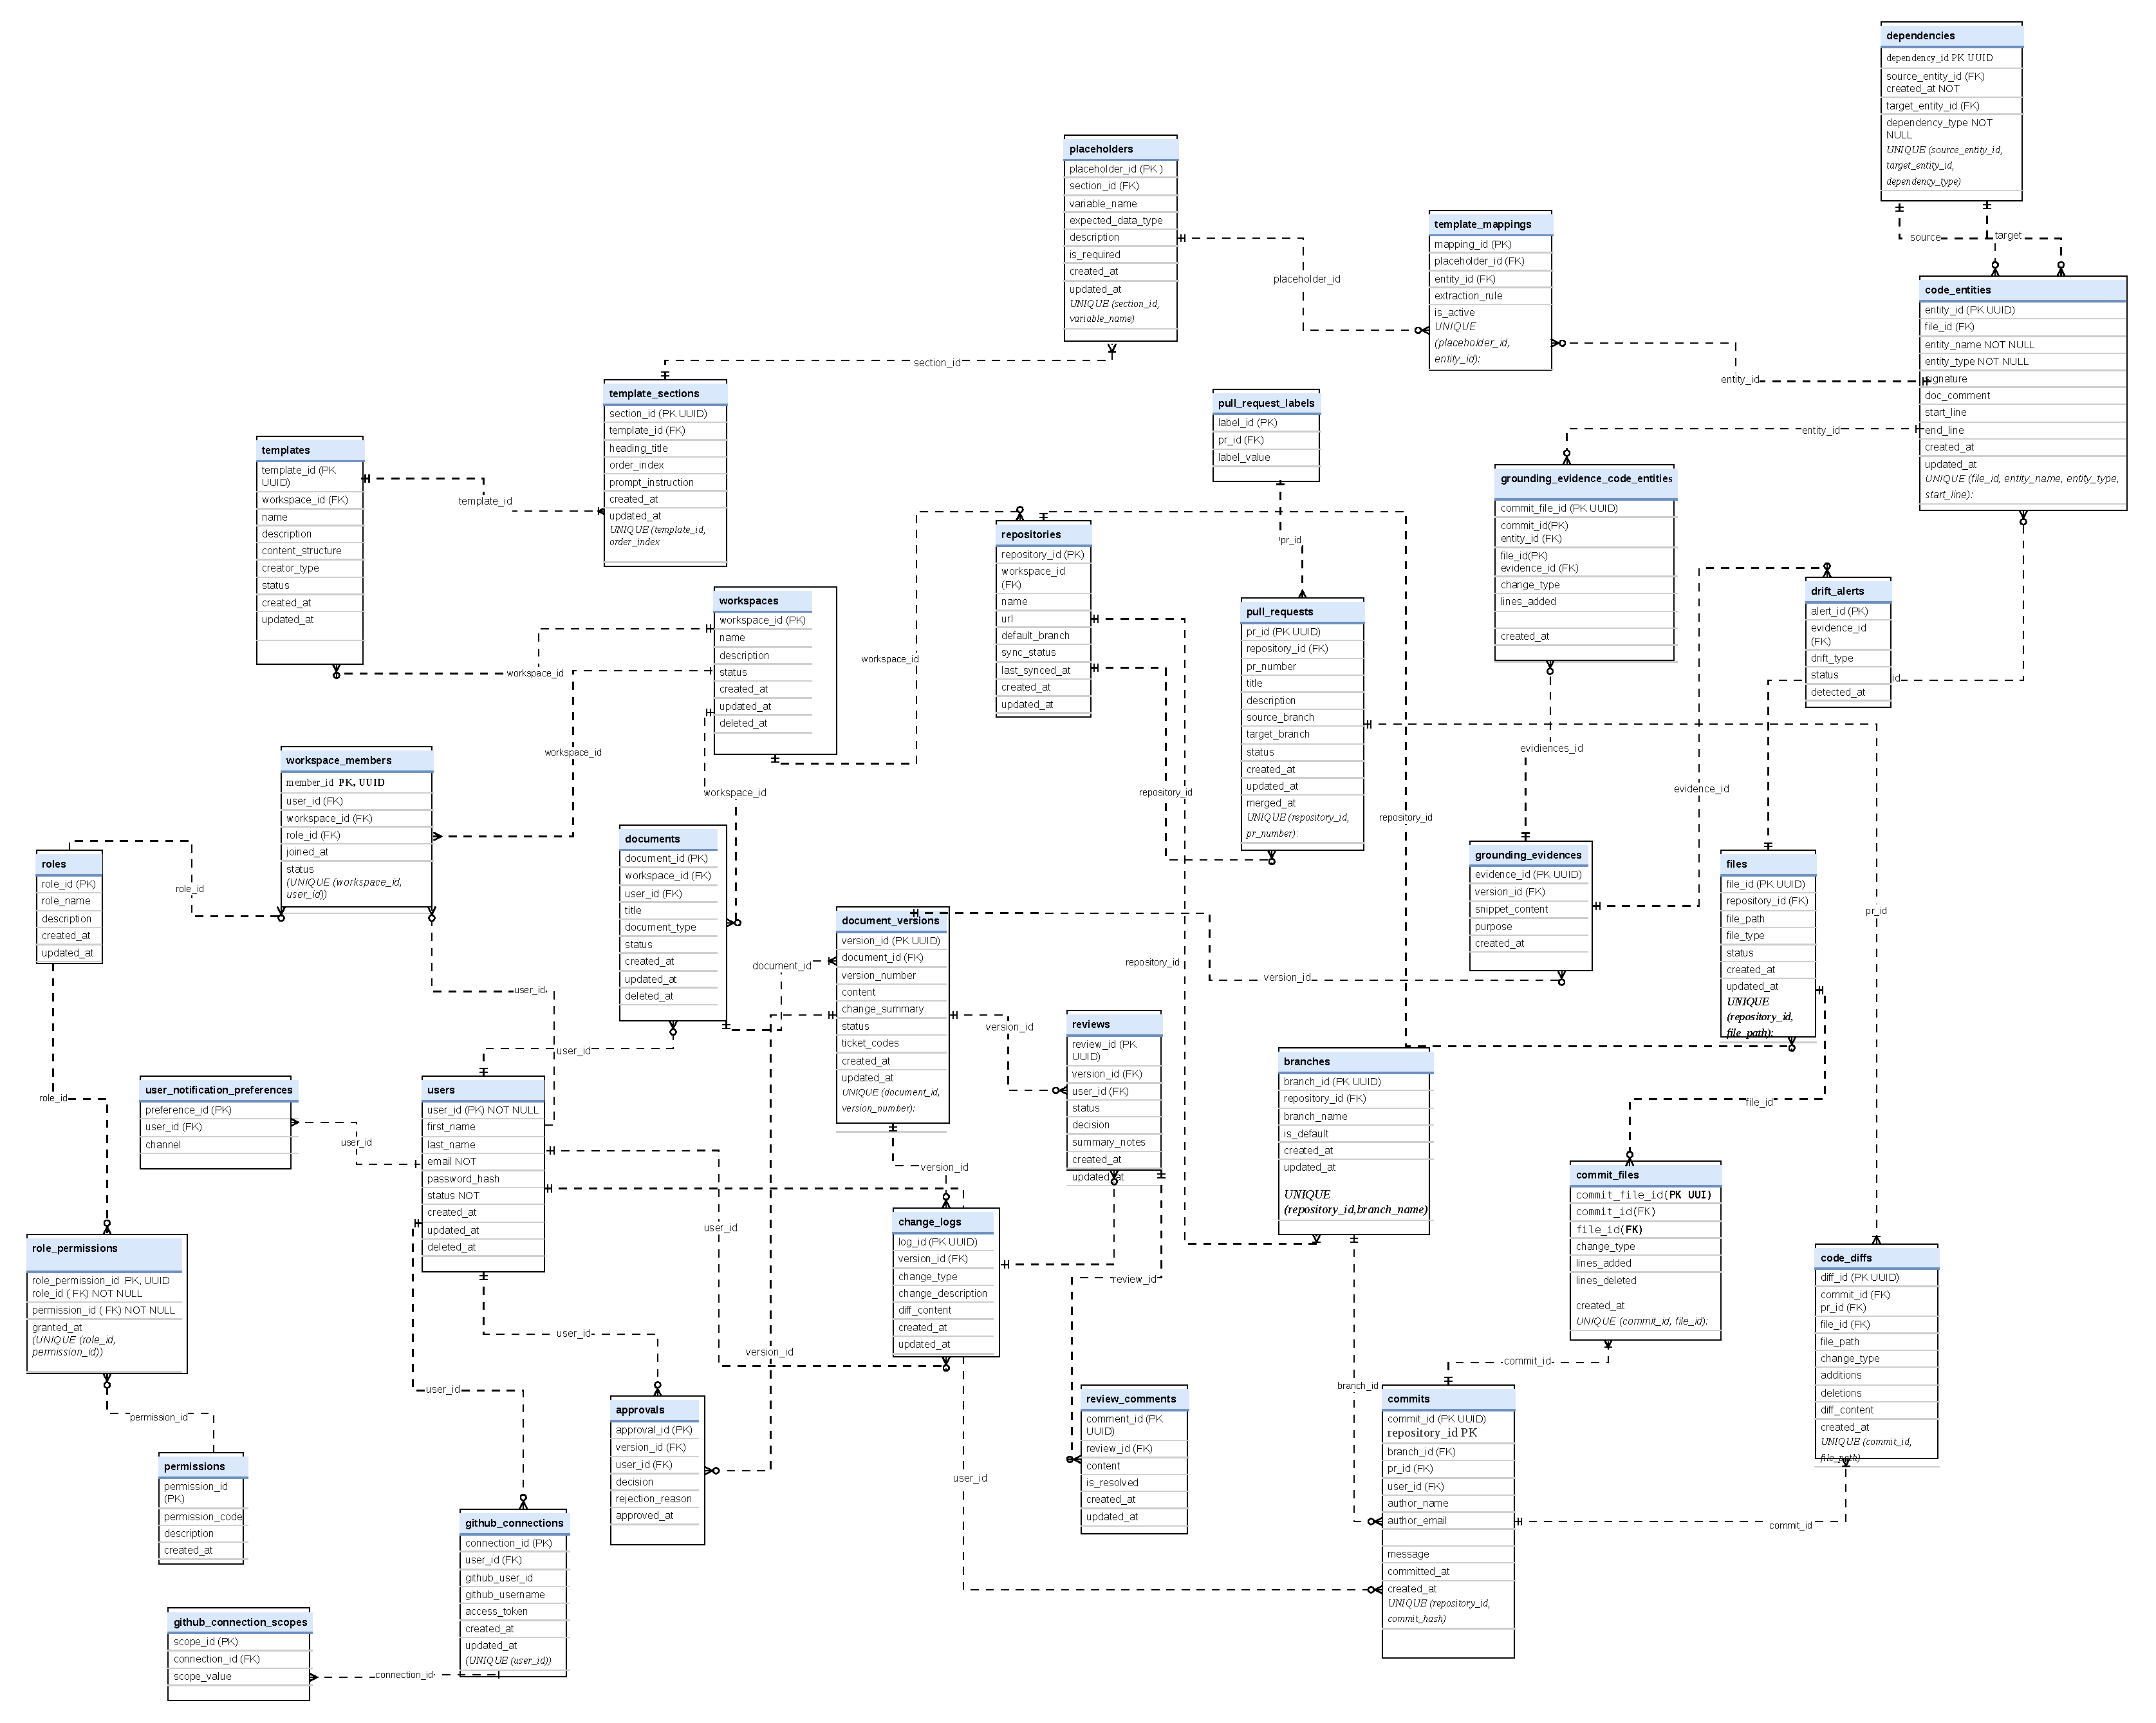
\includegraphics[
        width=\textwidth,
        height=0.75\textheight,
        keepaspectratio
    ]{./images/erd_muc_logic.pdf}
    \caption{Sơ đồ ERD mức logic}
    \label{fig:erd-logic}
\end{figure}